\documentclass[10pt,twoside]{article}

\usepackage{livreta5}


\usepackage{bookmark}
\usepackage{hyperref}
\usepackage{amssymb}
\usepackage{listings}
\usepackage{lscape}

\serie{S4 - Mathématiques}
\titre{Théorie des langages}
\soustitre{notes de cours \\
\small version du \today}
\auteurs{michel billaud \\ département informatique \\ iut de bordeaux}

\providecommand{\abs}[1]{|#1|}

\begin{document}

% \pagestyle{fancy}


\maketitle

\newpage

\section*{Avant-Propos}

Ce document contient mes notes personnelles pour préparer un cours de
Théorie des Langages de 16 heures (sur 4 semaines) 
destiné aux étudiants de 2ème année d'IUT
Informatique, au printemps 2014.

Il s'est trouvé que le programme pédagogique national (PPN) a changé
récemment, et que ce cours donné traditionnellement au semestre 4
(seconde année) est maintenant fait au semestre 2. Pendant l'année de
transition, il fallait faire ce cours en première année du nouveau PPN
et en deuxième année de l'ancien. Il se trouve qu'en plus il fallait
remplacer le collègue mathématicien qui assurait jusque-là ce cours,
c'était l'occasion de me remettre à la théorie des langages.

Malgré le volume horaire restreint (16h), j'ai décidé de parler un peu des
langages algébriques qui passent souvent à la trappe en DUT. Il me
parait important de faire le lien avec la syntaxe (et la compilation)
des langages de programmation, qui est quand même la motivation
principale pour faire ce cours en DUT, du point de vue des
informaticiens...


Dans ce cours, j'ai essayé de montrer un lien avec les applications
relative traditionnelles à la programmation : automates de reconnaissance
syntaxique, analyse des langages de programmation, ... tout en
montrant des techniques mathématiques nouvelles (pour les étudiants) :
travailler dans un produit cartésien (intersection de langages
rationnels), dans l'ensemble des parties d'un ensemble
(déterminisation), principe des tiroirs et des chaussettes (pour montrer
que $\{a^n b^n\}$ n'est pas rationnel), etc.

En tout cas j'ai eu plaisir à préparer ce cours, même pour une seule
fois, et j'espère ne pas avoir trop traumatisé mes étudiants !

\newpage



\tableofcontents
\clearpage

\part{Pour commencer}

\section{Motivations}

\subsection{Linguistique}

La \emph{théorie des langages} est issue de problématiques
de linguistique, pour l'étude de la structure des langues naturelles.

Une problématique était d'identifier des structures, comme par exemple
la décomposition d'une phrase en groupe sujet/groupe verbal/complément,
structures qui peuvent être communes à des groupes de langues

Remonter à une ``langue originelle'' et/ou identifier des mécanismes innés
communs à l'espèce humaine, qui prédisposeraient à l'usage d'une langue.


\subsection{Langages informatiques}

À la fin des années 50 sont apparus les premiers langages de
programmation. Au début, la programmation consistait à établir des
listes d'instructions machine, mais assez rapidement est apparu le
besoin d'écrire des programmes sous une forme plus ``naturelle'', dans
laquelle les éléments (fonctions, instructions, déclarations,
expressions, etc) sont combinés selon des règles précises.

Avec cela, la \emph{définition du langage}, vient une autre
préoccupation : comment écrire, à moindre frais, des
\emph{compilateurs} qui analysent le code source, et génèrent sa
traduction ?


Inversement, peut-on identifier des familles de langages faciles à
analyser ?

Applications
\begin{itemize}
\item reconnaissances des expressions régulières
\item automatiser la fabrication des compilateurs, en fournissant une
description du langage à reconnaître à un \emph{méta-compilateur}, qui 
produira un compilateur.
\end{itemize}

\subsection{Développements mathématiques}

Au delà de ces motivations pratiques, 
la \emph{théorie des langages} s'intéresse aux propriétés
mathématiques
des \emph{langages formels}.

C'est un domaine de l'informatique théorique
qui a connu une très grande activité à partir des années
70.

\section{Langages formels}

\subsection{Alphabet, lettres, mots}

\paragraph{Définitions et notations}

\begin{itemize}
\item
Un \textbf{alphabet} $A = \{a, b, c ...\}$,
est un ensemble fini\footnote{dans le cadre de ce cours}
de \textbf{lettres}.
\item
Traditionnellement, les lettres sont notées $a, b, c \ldots$,
et les variables qui parlent des lettres sont $x, y, z \ldots $
\item un \textbf{mot} $n$ est une séquence finie 
$(x, y, \ldots z)$ de lettres. On note un mot tout simplement en juxtaposant
ses lettres, soit $x y \ldots z$. 
\item $u, v, w$ désignent généralement des mots ($w$ comme word)
\item la \textbf{taille} d'un mot $w$ se note $\abs{w}$, c'est la 
longueur de sa séquence de lettres.
\item la lettre $\epsilon$ désigne le \textbf{mot vide}, de taille nulle. 
\item $A^n $
 désigne l'ensemble des mots de longueur $n \in \mathbb{N}$, 
\item $A^* = \bigcup_{i \in \mathbb{N}} A^i
=  A^0 \cup A^1 \cup A^2 \cup \ldots$ l'ensemble de tous les mots  sur  $A$.
\end{itemize}

\paragraph{Exemples} 

\begin{itemize}
\item soit $A$ l'alphabet à trois lettres $A = \{ a, b, c \}$
\item $a$, $bc$, $aaa$ sont des mots de longueurs 
respectives 1, 2 et 3 sur $A$
\end{itemize}

\subsection{Concaténation, facteurs}

\begin{itemize}
\item
\textbf{La concaténation} de deux mots consiste à les mettre bout à bout. 
Plus formellement,
si $u = x_1 x_2 \ldots x_n$ et $v = y_1 y_2 \ldots y_p$ sont deux mots
de longueurs respectives $n$ et $p$, le mot $u.v$ (noté aussi $uv$)
est la séquence $ x_1 x_2 \ldots x_n y_1 y_2 \ldots y_p$ de longueur
$n+p$.
\end{itemize}


\paragraph{Exercice. } La concaténation 
\begin{itemize}
\item est-elle associative ?
\item est-elle commutative ?
\item a-t-elle un élément neutre ?
\end{itemize}


\begin{itemize}
\item $u$ est dit \textbf{préfixe} de $w$ si il existe un $v \in A^*$
  que $uv = w$, c'est-à-dire que les lettres de $u$ sont identiques
  aux premières lettres de lettres de $w$.
\item De la même façon, $v$ est dit \textbf{suffixe} de $w$ si il
  existe un $u \in A^*$ que $uv = w$,
% \item le mot $f$ est un \textbf{facteur} d'un mot $w$ si $\exists
% u,v$ tels que $w = u f w$
\end{itemize}

\paragraph{Propriété}. Soit trois  mots $u, v, w$. on a équivalence entre
\begin{enumerate}
\item $ u v = u w $
\item $ v u = w u $
\item $ v = w $
\end{enumerate}


\paragraph{Le lemme de Levi} est un petit résultat utile dans les preuves :

Lemme : Si $u$ et $v$ sont des préfixes d'un même 
mot $w$, alors l'un d'eux est un préfixe de l'autre.


\paragraph{Preuve par cas,} selon l'ordre des longueurs. 
Idée : si $\abs{u} \leq \abs{v}$, les lettres de $u$ sont identiques
aux $\abs{u}$ premières lettres de $w$ qui sont identiques aux
premières lettres de $w$, donc $u$ est un préfixe de $v$.

\paragraph \textbf{Le théorème de commutation} est un peu plus surprenant

\paragraph{Théorème.} Deux mots commutent si et seulement si ils sont 
tous deux la répétition d'un facteur commun.

Autrement dit $ uv=vu $ si et seulement si il existe un mot $f$ et des
entiers $n$ et $p$ tels que $u=f^n$ et $v=f^p$.

\paragraph{Preuve}
\begin{itemize}
\item Évident dans un sens, puisque  $f^n f^p = f^{n+p} = f^{p} f^n$
\item Dans l'autre sens, par récurrence sur $N = \abs{u} + \abs{v}$.
\begin{itemize}
\item vrai dans le cas de base, quand $N = 0$, alors $u = v =
  \epsilon$,  commutent et sont une répétition de $\epsilon$.
\item si $\abs{u} = \abs{v}$, la commutation $uv = vu$ entraîne que $u = v$
\item sinon, comme $u$ et $v$ sont des préfixes de $uv=vu$, l'un est préfixe 
(strict) de l'autre. On suppose que c'est $u$, 
il existe donc $w$ tel que $v=uw$. L'égalité
$$uv = vu$$
s'écrit aussi 
$$u(uw) = (uw)u$$
qui se simplifie (voir plus haut) en 
$$uw = wu$$
Par hypothèse de récurrence, $u$ et $w$ sont des répétitions 
d'un même facteur $f$, et il en est donc de même pour $v=uw$, cqfd.
\end{itemize}
\end{itemize}


\subsection{Langages}

\paragraph{Définition} Un \textbf{langage} est un ensemble de mots.

\paragraph{Exemples} 
\begin{itemize} 
\item le langage des mots de deux lettres au plus sur $A = \{a, b\}$
  est $$L = \{ \epsilon, a, b, c, aa, bb, cc, ab, ba, bc, cb, ac, ca
  \}$$
\item $ \{ a^n \| 2 \leq n\leq 4\} = \{ aa, aaa, aaaa \}$
\end{itemize}

\subsection{Opérations sur les langages}

\paragraph{Opérations ensemblistes : } les langages sont
 des ensembles (de mots), on peut en faire
\begin{itemize}
\item l'intersection : par exemple si $L_1$ est l'ensemble des mots
  qui commencent par la lettre $a$, et $L_2$ ceux qui finissent par
  $b$, $L_1 \cap L_2$ contient les mots qui commencent $a$ \emph{et}
  finissent par $b$.
\item l'union, souvent notée $+$ : $L_1 + L_2$ contient les mots qui
  commencent $a$ \emph{ou} finissent par $b$ (ou les deux);
\item la différence, etc.
\end{itemize}

\paragraph{Le \emph{produit} de deux langages} est une opération 
spécifique, notée par un point : $L_1 . L_2$ est l'ensemble des mots
qui sont obtenus par concaténation d'un mot de $L_1$ avec un mot de
$L_2$.  Exemple : avec $L_1 = \{a, ab, c \}$ et $L_2 = \{ \epsilon, b
\}$
$$L_1.L_2 = \{ a, ab, c, abb, cb \}$$


\paragraph{L'élévation à une puissance  $L^n$} d'un langage $L$ 
consiste à concaténer $n$ mots de $L$.  Par exemple $\{a,ab\}^2 = \{
aa, aab, aba, abab \}$

\paragraph{L'étoile $L^n$} est l'union de tous les $L^n$, 
pour $n \geq 0$ : c'est l'ensemble des mots que l'on peut décomposer
en une suite de facteurs pris dans $L$. Il contient le mot vide, même
si celui-ci n'est pas dans $L$.

Ceci rejoint la notation  $A^*$ pour le langage de tous les
mots sur $A$.

\subsection{Comment définir  un langage ?}

\begin{itemize}
\item  par une \textbf{spécification}: l'ensemble des mots de 3 lettres sur 
$A = \{a, b \}$,
\item par un \textbf{algorithme qui produit tous les mots} du langage. 
\item par un \textbf{algorithme qui détermine si le mot appartient au langage}
\end{itemize}

\paragraph{Exercice : } quel langage est produit par l'algorithme suivant ?
\begin{verbatim}
pour n de 0 à l'infini, faire
 | pour i de 0 à n faire 
 |   |  w = epsilon
 |   |  pour j de 0 à i faire 
 |   |    | w = w.a
 |   |  pour j de i+1 à n faire
 |   |    | w = w.b
 |   |  afficher w
\end{verbatim}


\paragraph{Exercice : } écrire un algorithme qui produit tous les mots 
qui ne contiennent qu'un seul a (et autant de b qu'on veut avant et après).

\paragraph{Exercice : } quel langage est reconnu par l'algorithme suivant ?
% a^* b^**
\begin{verbatim}
donnée : w, mot sur {a,b}
booléen t = faux
pour toute lettre x de w, faire 
 | si x == b,  alors 
 |     | t = vrai
 | sinon si t alors
 |     | retourner faux
retourner vrai
\end{verbatim}
 
\paragraph{Exercice :} algorithme qui reconnaît le langage des mots sur 
$\{a, b, c\}$ qui ont exactement autant de $a$ que de $b$.

\paragraph{Exercice :} quel langage reconnaît cet algorithme ?
\begin{verbatim}
donnée w
entier c = 0
pour toute lettre x de w, faire 
 | selon x :
 |   si c'est un a, alors c++
 |   si c'est un b, alors c--
 | si c < 0, retourner faux
retourner vrai
\end{verbatim}

\subsection{Reconnaissance de motifs}

En utilisant le \emph{shell}, vous faites abondamment usage des
méta-caractères ``jokers'' \texttt{*} et \texttt{?}. Exemple
\begin{verbatim}
    a2ps  *.cc
    cp    prog-v?.*  archives
\end{verbatim}

Une chaîne correspond à un \emph{motif} comme \texttt{prog-v?.*},
si
\begin{itemize}
\item les caractères normaux sont identiques,
\item un joker \texttt{?} correspond à n'importe quel caractère,
\item un joker \texttt{*} correspond àà n'importe quelle chaîne.
\end{itemize}

\subsubsection{Backtracking}

L'examen du motif et de la chaîne à reconnaître se fait en parallèle.
Quand le caractère du motif est une étoile, il y a deux possibilités
\begin{itemize}
\item supposer qu'elle représente la chaîne vide, et examiner la même chaîne
avec le reste du motif
\item suppose qu'elle ``avale'' au moins un caractère du mot et reprendre
l'examen
\end{itemize}

On peut formaliser l'algorithme de façon récursive, et séparant les cas : motif
vide ou non, commençant par un point d'interrogation, un étoile ou autre chose,
et chaîne vide ou non.

\begin{lstlisting}
prédicat : reco (m , c)  où m est un motif
                         et c une chaîne
début
  selon que
   m est vide =>  voir si  c est vide 
   m est x.m' =>  voir si  c est y.c',  x==y  et
                           et reco (m', c')
   m est ?.m' =>  voir si  c est y.c'
                           et reco (m', c')
   m est *.m' =>  voir si  reco(m', c) 
                           ou  c est y.c'
                               et reco(m, c')
fin
\end{lstlisting}


Voici l'arbre de calcul pendant le déroulement de l'appel à
\texttt{reco("a*b", "aaba")}. 

Quand le motif commence par une étoile, 
il y a deux possibilités, soit on considère que l'étoile correspond
à une sous-chaîne vide (on enlève l'étoile du motif, sous-arbre de gauche),
 soit qu'elle 
``mange'' au moins un caractère de la chaîne (sous-arbre de droite).



\begin{center}
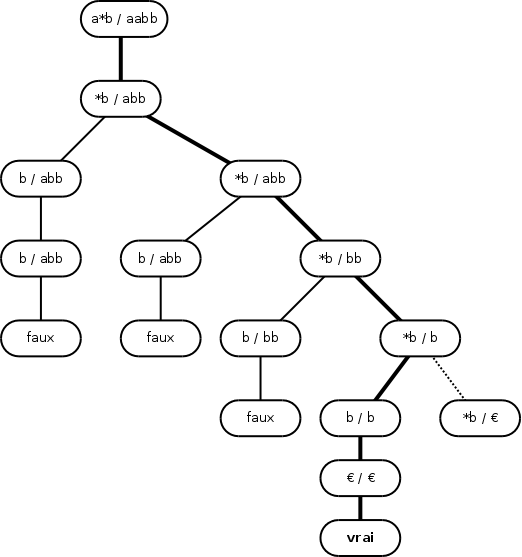
\includegraphics[width=\linewidth]{../dia/arbre}
\end{center}
On a là un exemple typique de procédure d'exploration d'un espace de
possibilités par \emph{backtracking} : on explore une alternative en
conservant la possibilité de revenir en arrière.

\subsubsection{Version récursive}

Le programme C++ suivant utilise la récursivité pour gérer le
backtracking par l'intermédiaire de la pile des appels.

\lstinputlisting[language=c++,frame=single,numbers=right]{../src/reconnait1.h}

Le programme est appelé ainsi :

\lstinputlisting[language=c++,frame=single,numbers=right]{../src/prog1.cc}
\subsubsection{Version itérative}

On peut faire mieux, en gérant explicitement une pile des alternatives restant
à explorer.

\lstinputlisting[language=c++,frame=single,numbers=right]{../src/reconnait2.h}


\subsection{Éviter le backtracking}

La problématique va être d'éviter ce backtracking, qui peut être
extrêmement coûteux en temps de calcul.

\paragraph{Exercice.} Calculez, en fonction de $n \in \mathbb{N}$ le nombre de noeuds de l'arbre de recherche
pour le motif "\texttt{*a}" et le mot $b^na$.

Pour reconnaître ces mots, il suffit d'un petit dessin  :

\begin{center}
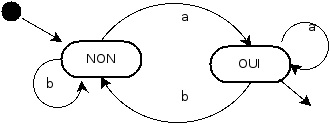
\includegraphics[width=.8\linewidth]{../dia/auto}
\end{center}



On part de l'état de gauche, on suit les flèches au fur et à mesure de la lecture des lettres du mot à reconnaître, et à la fin on sait que le mot est reconnu si on est arrivé dans l'état OUI. C'est la notion d'automate

\clearpage

\part{Langages rationnels}

\section{Automates finis déterministes}

\subsection{Définition}

\paragraph{Un automate} $\mathcal{A}$ est la donnée
\begin{itemize}
\item d'un alphabet $A$ (fini)
\item d'un ensemble fini d'\textbf{états} appelé traditionnellement $Q$
\item d'un \textbf{état initial} $q^I \in Q$,
\item d'un ensemble $Q_F \subseteq Q$ d'\textbf{états finaux} (ou terminaux);
\item d'une \textbf{fonction de transition} $\delta : Q \times A \rightarrow Q$
\end{itemize}


Les automates se prêtent à une représentation sous forme de
graphes. Les états sont des noeuds, les transitions des flèches entre
les noeuds, portant l'étiquette de la lettre.

L'état initial est indiqué par un point, ou une flèche entrante. 
Les états finaux
le sont par un double cercle, un triangle, une flèche sortante ...

\paragraph{Un mot est reconnu} par un automate si, en partant de l'état initial
et en suivant les transitions qui correspondent aux lettres successives du mot,
on arrive dans un état final.

Plus formellement, à partir d'un $w$ un mot de longueur $n$ on construit 
une séquence de $n+1$ états $(q_0, q_1, \ldots, q_n)$ avec
\begin{itemize}
\item $q_0 = q^I$ (l'état initial)
\item $q_i = \delta(q_{i-1}, w_i)$, pour tout $i$ entre 1 et $n$
\end{itemize}
$w$ est reconnu si et seulement si le dernier état est final, soit
$q_n \in Q_F$.


\subsection{Quelques exemples}



\subsection{Comment coder un automate}

Un automate peut aisément être codé par un tableau (constant) à deux dimensions. 
La première dimension correspond à l'état 
et la seconde les catégories de caractères en entrée.

Pour noter les états et les catégories, on peut faire usage d'énumérations.


\lstinputlisting[language=c++,frame=single,numbers=right]{../src/automate.cc}


\subsection{Un exemple plus détaillé}

Construction d'un gros exemple : reconnaissance d'une ligne de fichier CSV

Le contenu d'une feuille de calcul (tableur) peut être exporté au format CSV
(comma-separated values), dans lequel
\begin{itemize}
\item les cellules d'une même ligne de la feuille sont représentées par une ligne de texte
\item si une case n'est pas vide, son contenu est entouré de guillemets,
\item les guillemets qui sont dans les cases sont doublés
\item les représentations des cases sont séparés par des virgules
\end{itemize}


Exemple, la rangée de cellules
\begin{center}
\begin{tabular}{|c|c|c|c|}
\hline
& 123 & route de paris & lieu dit "Le bourg" \\
\hline
\end{tabular}
\end{center}


est codée par la ligne
\begin{verbatim}
,"123","route de paris","lieu dit ""Le bourg""""
\end{verbatim}
On demande de construire une fonction qui détermine si une ligne de texte est valide ou non.


\subsection{Applications}

Définissez des automates pour les applications suivantes

\paragraph{Vérifier la ponctuation d'un texte  : }  en français une ponctuation
double, comme deux-points ou point-virgule, doit être précédée et
suivie d'un ou plusieurs espaces, contrairement aux ponctuations
simples (espaces après mais pas avant).  Faire un automate qui vérifie
la ponctuation d'une ligne de texte (qui ne peut pas commencer par une
ponctuation, même précédée d'espaces).

On travaillera sur un alphabet $A=\{e, s, d, l\}$ de catégories de caractères : 
$e$ pour les espaces, $s$ et $d$ pour les ponctuations simples et doubles, $l$ pour les lettres.


\paragraph{Vérifier une chaîne de caractères en C : } Une chaîne 
de caractère en C est entourée
par des guillemets. Si on doit coder des guillemets à l'intérieur, on
les précède par un ``backslash''.  Si on doit représenter un
backslash, on le double.  On travaillera sur un 
alphabet $A=\{g, b, a\}$ de catégories de caractères : $g$ pour les guillemets, $b$ pour
backslash, $a$ pour les autres.



\subsection{Langages rationnels}

\paragraph{Définition. } Un langage est dit \textbf{rationnel} si il existe
un automate qui le reconnaît.

Les langages rationnels constituent une des familles les plus importantes
de la hiérarchie définie par Chomsky.

Quelques propriétés :
\begin{itemize}
\item La famille des langages rationnels sur un alphabet $A$ est close
  par par complément, union, intersection, différence (voir ci
  dessous) étoile (preuve plus tard, avec les automates
  non-déterministes)
\item on peut déterminer si deux automates reconnaissent le même langage
(par un calcul sur les automates)
\item on peut calculer  (automatiquement)
un automate minimal.
\end{itemize}

\subsection{Un langage qui n'est pas rationnel}

Tous les langages ne sont pas rationnels, mais encore faut-il le prouver.
L'exemple classique est  $L = \{ a^n b^n, n \in \mathbb{N} \}$

L'idée de la preuve, c'est que pour reconnaître si un mot est dans L,
il va falloir compter combien on a rencontré de $a$, pour voir ensuite 
si on a
autant de $b$. Le seul moyen de compter, c'est d'être dans des états
différents. Comme le nombre d'états est fini, on ne peut pas y
arriver.




\paragraph{Preuve par l'absurde}
\begin{enumerate}
\item on suppose qu'il existe un automate à $N$ états qui reconnaît
  $L$, et on considère le mot $a^N b^N$ qui est dans $L$.
\item on regarde le parcours dans l'automate pendant la reconnaissance du
préfixe $a^N$. On part de l'état initial, et on fait $N$ ``pas''.
\item Par le principe de poteaux et des intervalles, on est donc passé par
$N+1$ états. 
\item Principe des tiroirs et des chaussettes : comme il n'y a que 
$N$ états distincts, on est forcement passé au moins deux fois au 
même endroit : on a donc fait une boucle de transitions étiquetées $a$, soit $B$ la longueur de cette boucle.
\item en partant de l'état initial, on arrive donc au même état que par $a^N$, en
faisant un tour de plus, c'est à dire par $a^Na^B = a^{N+B}$
\item de là,  suivre $N$ transitions  ``b''  mène à un état terminal, 
puisque $a^Nb^N$ est reconnu.
\item donc $a^{N+B}b^N$ est également reconnu par l'automate.
\item Or il ne fait pas partie du langage : c'est une contradiction.
\end{enumerate}


\subsection{Complément d'un langage rationnel}

Il est facile de voir que le complément (par rapport à $A^*$) d'un langage
rationnel $L$ sur $A$ est lui-même rationnel.


\paragraph{Preuve}
\begin{enumerate}
\item $L$ est rationnel, il existe un automate $\mathcal{A}$ qui le reconnaît.
\item construisons $\mathcal{A'}$ identique à $\mathcal{A}$, avec les mêmes états,
les mêmes transitions, le même état initial, mais en prenant comme états
terminaux ceux qui ne le sont pas dans $\mathcal{A}$ :
$ Q'_F = Q \setminus Q_F$.
\end{enumerate}
Ainsi, les mots reconnus par $\mathcal{A'}$ sont ceux qui ne sont pas dans $L$,
et inversement. Le langage $L'$ reconnu par $\mathcal{A'}$ est le complément de $L$.

\subsection{Intersection et Union, automate produit}

\label{union}

Montrons maintenant que l'intersection de deux langages rationnels 
 $L_1$ et $L_2$ est elle-même rationnelle.

\paragraph{L'idée intuitive} est très simple : pour voir si un mot $w$ appartient 
à \textbf{l'intersection} $L_1 \cap L_2$,
on utilise deux automates $\mathcal{A}_1, \mathcal{A}_2$ qui reconnaissent
$L_1$ et $L_2$.

Jusqu'ici, on reconnaissait un mot en pointant du doigt l'état initial, et en suivant les flèches correspondant aux lettres. Le mot est reconnu si on s'arrête sur
un état final.

Maintenant on fait la même chose avec deux doigts, un par automate. Au départ on 
pointe la paire d'états initiaux, et on progresse simultanément dans les deux automates. Le mot est reconnu si on s'est arrêté sur une paire d'états finaux.

On travaille donc sur des \textbf{paires d'états} des deux
automates. C'est la notion de produit d'automates.

\paragraph{Plus formellement,} on construit ainsi le produit  $\mathcal{A}$ qui reconnaît l'intersection
\begin{itemize}
\item l'alphabet $A$ est le même,
\item l'ensemble $Q$ des états est le produit cartésien $Q_1 \times  Q_2$,
\item l'état initial est la paire  d'états initiaux $({q^I}_1, {q^I}_2)$
\item les états finaux sont les paires d'états finaux des automates $Q_F = {Q_1}_F \times  {Q_2}_F$,
\item la fonction de transition $\delta$ combine les transitions dans les deux automates
$$ \delta( (q_1, q_2) , x ) = ( \delta_1(q_1, x), \delta_2(q_2, x)) $$
pour toute lettre $x \in A$, et pour tous états $q_1 \in Q_1,  q_2 \in Q_2$. 
\end{itemize}

On notera que cette construction peut faire apparaître des états inaccessibles
depuis l'état initial. On peut les ignorer.

\paragraph{Exercice.} Donnez des automates pour 
\begin{itemize} 

\item $L_1$  les mots qui commencent par $a$.
\item $L_2$  les mots qui finissent par $b$.
\item $L_3$ = $L_1 \cap L_2$
\item $L_4$ mots qui  contiennent au moins deux $a$ consécutifs,
\item $L_5$ = = $L_3 \cap L_4$
\end{itemize}

\paragraph{Pour l'\textbf{union} de deux
langages rationnels} la construction est similaire : un mot est
reconnu si on arrive dans un état final pour au moins l'un des
automates.

Autrement dit on prend comme états terminaux l'ensemble
$$Q_F = ({Q_1}_F \times Q_2)  \cup  (Q_1 \times {Q_2}_F)$$.


\subsection{Concaténation de langages}

Il est  tentant de vouloir appliquer la même idée pour déterminer
si un mot $w$ appartient à la concaténation de deux langages $L_1$ et $L_2$ :
on part de l'état initial du premier automate, et on le suit jusqu'à obtenir un
état final. Puis on part de l'état initial du second, et on continue avec les lettres qui restent.

Mais malheureusement ce n'est pas aussi simple : il peut y avoir 
plusieurs préfixes $u$ de $w$ qui conduisent à des états finaux de $\mathcal{A}_1$ : a priori 
on ne sait pas pour lequel il faut choisir de passer dans le second automate.

Pour aborder ces problèmes, nous allons donc introduire une généralisation de la notion d'automate
: les \textbf{automates non déterministes avec $\epsilon$-transitions}.

Nous verrons que si cette notion est plus générale, et permet
d'exprimer plus facilement les idées (notamment la reconnaissance d'un
produit de langage, ou l'étoile d'un langage), en fait on peut
toujours les ramener à des automates déterministes qui reconnaissent
le même langage.

\clearpage
\section{Automates non déterministes}


\subsection{Un automate non-déterministe} $\mathcal{A}$ sur un alphabet $A$
est la donnée de 
\begin{itemize}
\item un ensemble d'états $Q$
\item un ensemble $Q_I \subseteq Q$ d'états initiaux
\item un ensemble $Q_F \subseteq Q$ d'états finaux
\item un ensemble $\Delta \subseteq (Q \times A \times Q)$  de transitions
\end{itemize}

Sur le schéma d'un automate, il y a donc éventuellement
\begin{itemize}
\item plusieurs entrées possibles au lieu d'une seule pour les automates déterministes
\item en partant d'un état, il peut y avoir plusieurs transitions concernant la même lettre, ou aucune.
\end{itemize}

\paragraph{Exemple : } dans l'automate ci-dessous, en lisant des $a$ depuis l'état 0, on peut rester dans 0, aller en 1 ou encore en 2. Par contre dans l'état 1, on ne peut aller nulle part en lisant un $b$. 


\begin{center}
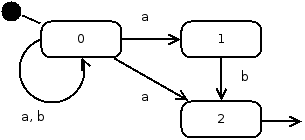
\includegraphics[width=.6\linewidth]{../dia/nondet}
\end{center}

\paragraph{Un mot $w$ est reconnu} par un automate non-déterministe 
si et seulement il existe un chemin dans l'automate
\begin{itemize} 
\item qui parte d'un état initial
\item qui soit étiqueté par les lettres successives du mot
\item qui mène à un état final
\end{itemize}

Sur l'automate, on voit assez facilement que pour aller de 0 à 2, il
faut un mot qui se termine par la lettre $a$ ou par le suffixe $ab$.


\paragraph{L'intérêt pratique} des automates non déterministes, 
c'est qu'ils sont plus faciles à concevoir que les automates non déterministes.

Exemple : définissez un automate qui reconnaît les mots qui se terminent par
$ababab$.

\subsection{Retour sur l'union}

En \ref{union}, nous avons vu une façon de construire un automate déterministe
qui reconnaît l'union de  deux langages rationnels.



\paragraph{Exemple : } construisez un automate reconnaissant les mots 
% qui contiennent le facteur $aa$. Même question pour $bab$.
% Même question pour ceux qui contiennent au moins un de ces facteurs.

\paragraph{Exercice : construire des automates non-déterministes} pour les mots sur $A = \{l,c,a\}$ (lettre, chiffre, autre)
qui reconnaissent
\begin{itemize}
\item les nombres entiers, suites d'au moins un chiffre,
\item les identificateurs (une lettre, suivie de lettres ou de chiffres)
\item les nombres et les identificateurs
\end{itemize}

\paragraph{La construction générale} de l'automate pour l'union.
\begin{itemize}
\item l'automate est l'union de deux copies distinctes des automates
\item états : union des deux ensembles d'états
\item états initiaux (resp. finaux) : union des deux ensembles d'états initiaux
(resp. finaux)
\item transitions : union des ensembles de transitions.
\end{itemize}


\subsection{Déterminisation}

En partant de l'état initial, la lettre $a$ fait passer dans l'état 0, l'état 1 ou l'état 2.

Ceci conduit à l'idée de considérer \emph{l'ensemble des états} où l'on peut se trouver après avoir lu une séquence de lettres, par exemple $abaa$
\begin{itemize}
\item au début on ne peut être que dans l'état initial, soit $\{0\}$ ;
\item le premier $a$ mène dans $\{ 0, 1, 2 \}$,
\item le $b$ dans $\{0, 2\}$,
\item le $a$ dans $\{ 0, 1, 2 \}$,
\item le dernier $a$ dans $\{ 0, 1, 2 \}$.
\end{itemize}

\begin{center}
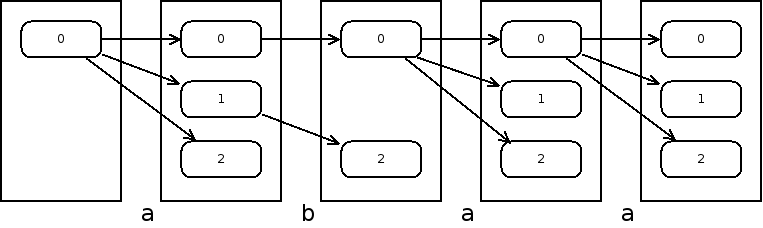
\includegraphics[width=.9\linewidth]{../dia/deroulement}
\end{center}


Parmi ces états se trouve un état terminal : le mot est donc reconnu.

\paragraph{Le procédé de déterminisation est donc simple} : partant 
d'un automate $\mathcal{A}$ non 
déterministe, on construit un automate déterministe  $\mathcal{A'}$ de 
la façon suivante :

\begin{itemize}
 \item les états sont les parties de $Q$ : $Q' = \mathcal{P}(Q)$
\item l'état initial regroupe tous les états initiaux : $q'_I = Q_I$
\item les états finaux sont ceux qui contiennent au moins un état final : 
$Q'_F =  \{ q' \in Q' | q' \cap Q_F \neq \emptyset \}$
\item la fonction de transition fait passer dans l'état qui 
regroupe tous les états accessibles par une lettre :
$\delta'(q', x) = \{ q_2 | \exists (q_1, x, q_2) \in \Delta, q_1 \in q'\} $ 
pour tout état $q' \in Q'$, et toute lettre $x \in A$.
\end{itemize}

En pratique,  on n'a pas besoin de calculer tous les 
états, seulement ceux qui sont accessibles depuis l'état initial.

\paragraph{Exercice :} déterminiser l'automate ci-dessus.

\paragraph{Conséquence :} les langages reconnus par les
automates non-déterministes sont rationnels (et inversement).


\subsection{Automates avec $\epsilon$-transitions}

En ajoutant des ``epsilon-transitions'', on donne la possibilité à 
l'automate, de passer d'un état à un autre ``spontanément'', sans lire 
de lettre.

Exemple, reconnaître les nombres formés de chiffres ($c$), qui commencent
 éventuellement 
par un signe ($s$). Les $\epsilon$-transitions sont représentées par des flèches en pointillés :
\begin{center}
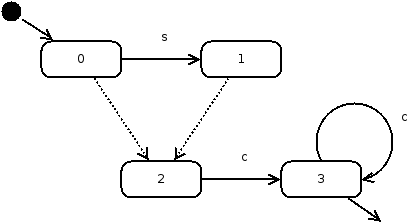
\includegraphics[width=0.6\linewidth]{../dia/nombre-signe-non-det}
\end{center}

Ces transitions apportent une facilité d'expression des idées.
Elles peuvent être éliminées (nous verrons comment) pour revenir
des automates non-déterministes ``simples'', qui eux-mêmes se ramènent
à des automates déterministes.

\paragraph{Conséquence.} Les automates non-déterministes
 avec $\epsilon$-transitions reconnaissent les langages rationnels.
 

\subsection{Concaténation de langages}

La construction d'un automate qui reconnaît la concaténation de 
deux langages, à partir de leurs automates, est simple :
\begin{itemize}
\item les états initiaux sont ceux du premier automate
\item les états finaux sont ceux du second
\item les transitions sont conservées
\item on y ajoute des $\epsilon$-transitions entre les états finaux du premier et les états initiaux du second
\end{itemize}


Voir sur l'exemple précédent, qui est le produit de deux langages
\begin{itemize}
\item celui qui reconnaît un signe facultatif
\item celui qui reconnaît une suite de chiffres.
\end{itemize}

\paragraph{Application : } faire un automate qui reconnaît les
nombres écrits en notation scientifique, comme par exemple 
$ -3.14E+23 $.  Ils comportent une mantisse et éventuellement un 
exposant (commençant par E). La mantisse a éventuellement un signe,
peut être entière ou décimale (mais si il y a un point décimal,
il y a au moins un chiffre à gauche ou à droite). L'exposant
 peut aussi être signé

\subsection{Étoile}

Et de même l'étoile d'un langage s'obtient, par exemple
\begin{itemize}
\item en ajoutant un état supplémentaire à l'automate, qui sera le 
seul état initial et final.
\item en ajoutant des $\epsilon$-transitions de cet état vers
les (anciens) états initiaux, et depuis les (anciens) états
finaux
\end{itemize}


\subsection{Élimination des $\epsilon$-transitions}

Pour tout automate avec $\epsilon$-transitions, on peut construire un
automate équivalent qui n'en a pas. Méthode
\begin{itemize}
\item pour chaque état $q$, on détermine l'ensemble $S(q)$ de ses
  successeurs, qui peuvent être atteints par une ou plusieurs
  $\epsilon$-transitions.
\item pour chaque transition ``normale'' qui mène à $q$, on ajoute une
  transition similaire (même origine, même lettre), vers tous les
  états de $S(q)$
 \item pour chaque transition ``normale'' qui part de $q' \in S(q)$,
   on ajoute une transition similaire partant de $q$ ( même lettre,
   même destination)
\item si $q$ est un état initial, tous les successeurs deviennent initiaux
\item si au moins un des successeurs de $q$ est final, $q$ devient final.
\end{itemize}

Cette méthode permet d'éliminer les ``raccourcis'' que sont les
$\epsilon$-transitions.

\paragraph{Application} : automate qui reconnaît si 
une ligne contient une suite de nombres entiers (éventuellement aucun)
Les entiers peuvent avoir des signes, ils sont séparés par
des espaces (au moins un). Il peut y avoir des espaces en début
et en fin de ligne.


\subsection{Conséquence : le théorème de Kleene}

Ce théorème célèbre dit que l'ensemble des 
langages rationnels, qui sont définis à
 partir des singletons (mots d'une lettre), et des unions, 
 produits et
 étoiles de langages rationnels, coïncide avec
 l'ensemble des langages reconnus par
 des automates finis. 
 
 Nous l'avons démontré par petits bouts, en introduisant
 des notions qui facilitent la preuve : automates 
 non-déterministes, $\epsilon$-transitions, mais qui peuvent
 toujours se ramener
 aux automates déterministes.
 
 En le combinant le théorème de Kleene avec 
 d'autres propriétés que nous avons
 déjà remarquées (par exemple 
 l'intersection et la différence de deux
 rationnels est rationnelle), cela fournit des arguments
 pour montrer qu'un langage est rationnel (ou pas).

\paragraph{Exemple :} le langage $L$ des mots sur $A = \{a, b \}$ qui
n'ont pas le même nombre de $a$ que de $b$ est-il rationnel ?
deux lettres.

Raisonnement :
\begin{enumerate}
\item si il l'était, son complémentaire $L_1$, 
qui contient les mots qui ont autant
de $a$ que de $b$, le serait aussi. 
\item L'intersection de $L_1$ avec un autre rationnel le serait aussi.
Soit $L_2 = L_1 \cap a^* b^*$
\item or $L_2 = \{ a^n b^n, n \in \mathbb{N}\}$, le fameux exemple
 de langage  qui n'est pas rationnel.
 \item donc $L$ n'est pas rationnel.
\end{enumerate}

\paragraph{Exercice : } montrer que le "langage des parenthèses" 
n'est pas rationnel.  Exemple de mot de ce langage : 
"\texttt{(()())()((()))}". En tout il y a autant d'ouvrantes 
que de fermantes,
et dans un préfixe il ne peut y avoir moins de fermantes 
que d'ouvrantes.

 \subsection{Quelques autres propriétés}
 
 Une application du théorème de Kleene, c'est que pour prouver
 une propriété des langages rationnels, on peut se ramener
 à des opérations sur les automates qui les reconnaissent.
 
\paragraph{ Exemples :}
 \begin{itemize}
 \item Le \textbf{miroir} $\widetilde{w}$ d'un mot $w_1 w_2 \ldots 
  w_n$ s'obtient 
 en inversant les lettres : $\widetilde{w} = w_n \ldots w_2 w_1$.
 Comment montrer que le miroir d'un langage 
 rationnel est lui-même rationnel ?
 \item Appelons $\gamma_x(w)$ le mot obtenu en effaçant de $w$ toutes
 les apparitions de la lettre $x$. 
 Par exemple $\gamma_a{aabcabbac} = bcbbc$. Comment montrer que 
 pour tout langage rationnel $L$ et pour toute lettre $x$, 
 $\gamma_x(L)$ est rationnel ?
 \end{itemize}
 
 \paragraph{Application :} on considère les expressions arithmétiques
 bien parenthésées, du genre "\texttt{3*(x-5)+1/(y*(z-3)}". 
 Est-ce un langage rationnel ?
 
\subsection{Cas pratiques}

\begin{enumerate}
\item 
Comment analyser des fichiers de configuration qui ressemblent à ceci :
\begin{verbatim}
;
; config
;
[database]
name = "mabase"
type = "mysql"
port = 2134
login = toto    ; à changer

[images]
directory = "/usr/local/images"
...
\end{verbatim}
donnez-en une description formelle complète.
\item 
Même question pour le langage de description d'automates ci-dessous
\begin{verbatim}
automate Premier
état ZERO initial
       a -> ZERO   b -> ZERO UN
état UN final

automate Second
état ZERO initial final  
       a -> ZERO UN
       b-> UN 
état UN  
      a -> ZERO
\end{verbatim}
\end{enumerate}

\clearpage
\section{Expressions régulières}

\subsection{Notion}

Un exemple : $ab(c^*) + (a+b)^*c$

Les \textbf{expressions régulières}
 sont un moyen de noter des langages en
partant
\begin{itemize}
\item de singletons comme $a$, $b$, $c$ et du mot vide ;
\item de l'étoile, du produit et de l'union (notée +) de langages.
\end{itemize}.
Les parenthèses servent à désambiguïser.
Comme vous le savez, ces opérations suffisent
 pour noter tous les langages 
rationnels.

Les expressions régulières sont aussi utilisées comme outil de 
programmation (bibliothèque \emph{regex}) pour valider des chaînes
de caractères, ou les découper en morceaux.

\subsection{De l'expression à l'automate}

La construction d'un automate (non déterministe) à partir
de l'expression régulière ne pose pas de difficulté.

\paragraph{Exercice :} application à l'exemple.

Elle peut d'ailleurs facilement être automatisée.

\subsection{De l'automate à l'expression régulière}

Beaucoup plus amusant : à partir d'un automate, on peut construire
une expression du langage, en utilisant le \emph{lemme d'Arden} 
(voir plus loin).

Rappelons que le langage reconnu par un automate, ce sont les mots
qui mènent d'un état initial  à un état final.

A chaque état $q_i$ (on suppose qu'ils sont numérotés), on associe le
langage $L_i$ des mots qui mènent de l'état $q_i$ à un état final.
L'automate reconnaît donc l'union des $L_i$, pour les $q_i \in Q_F$.

Observons les chemins qui partent d'un état $q_i$
\begin{itemize}
\item si $q_i$ est final, alors  $\epsilon \in L_i$
\item si il y a une transition $x$ de $q_i$ à $q_j$, alors
$L_i \supseteq x L_j$ : parmi les chemins qui vont de $q_i$ à un état 
terminal, il y a ceux qui partent de $q_j$, après un premier pas $x$.
\end{itemize}

Plus précisément on a une équation pour chaque état final
$$ L_i = \bigcup_{(q_i,x,q_j) \in \Delta} x L_j  \cup \{\epsilon\}$$
et pour chaque état non final 
$$ L_i = \bigcup_{(q_i,x,q_j) \in \Delta} x L_j $$

Ceci permet de traduire un automate non-déterministe 
en système d'équations portant sur les langages

Exercice : de quel automate viennent ces équations ?
\begin{eqnarray*}
L = L_1 &=& (a + b) L_1 + b L_2 \\
L_2 &=& b L_2 + \epsilon
\end{eqnarray*}
 
Pour résoudre ce système, on applique les bonnes vieilles méthodes
de substitution et d'élimination.

Intuitivement (et en regardant l'automate), $L_2$ est une suite, 
éventuellement vide de $b$. Autrement dit $L_2 = b^*$.

Donc en substituant :
$$ L_1 = (a + b) L_1 + b b^* $$
et là encore, intuitivement, $L_1$ est une répétition de $a$ ou de $b$
suivie par une répétition d'au moins un $b$.
$$ L_1 = (a + b)^* + b b^* $$

pour ce faire nous avons utilisé un petit résultat : le lemme d'Arden

\subsection{Résultat : le lemme d'Arden}

\paragraph{Lemme :} soient $B$ et $C$ deux langages rationnels : 
la plus petite solution de l'équation 
$$ X = BX + C $$
est le langage $X = B^* A$. Et c'est l'unique solution si
$\epsilon \not\in B$.


\paragraph{Remarque. } Que se passe-t-il quand $\epsilon \in B$, par exemple
le cas particulier de l'équation $X = X + C$ ? 
Alors dans ce cas il n'y a pas
\emph{une seule} solution : tout ensemble est solution si et seulement
si il contient $C$. À partir du moment où $\epsilon \in B$, 
l'ensemble $A^*$ de tous les mots est également solution. En mathématiques,
dans ce type de situation, on recherche - si c'est possible -  la plus
petite (ou la plus grande) solution.

\paragraph{Preuve}
\begin{itemize}
\item $B^* C$ est toujours solution de l'équation parce qu'on a
la propriété $L^* = LL^* + \epsilon$ pour tout langage $L$.
En
 remplaçant en partie droite, 
 \begin{eqnarray*}
 BX+C &=& B(B^* C) + C \\ 
      &=& (B B^*)C + \epsilon C \\
      &=& (B B^* + \epsilon) C \\
      &=&  B^* C
      \end{eqnarray*}
\item on montre très facilement que 
toutes les solutions contiennent 
$ B^* C = B^0 C + B^1C + B^2 C + \ldots$.

Soit $S$ tel que $S = BS+C$. Alors en remplaçant successivement
$$\begin{array}{rccccl}
 S &=& B S + C \\
 = B^1 S + B^0 C &=& B^1 (B S + C) + B^0 C \\
    =  B^2 S + B^1 C + B^0 C &=&  B^2 (BS+C) + B^1 C + B^0 C \\
    = B^3 S + B^2 C+ B^1 C + B^0 C &=& \ldots
\end{array}
$$

Donc $S$ contient tous les ensembles $B^nC$ et donc $B^*C$ qui est
leur union. 
\item si $B$ ne contient pas $\epsilon$, tout mot de $B$ a au moins 
une lettre, et un mot $w$ de longueur $n$ ne peut pas appartenir
à $B^{n+1} L$ où L est un langage quelconque.

Or une solution $S$ se "déplie" en
$$ S = B^{n+1}S + B^nC + B^{n-1}C + \ldots + B^0 C$$
et si $w$ de longueur $n$ appartient à $S$, il appartient
forcément à un des $B^k C$, et donc à $B^*C$ qui est leur union
pour tout $k$ entier. Donc tout mot $w$ de $S$ appartient à $B^*C$, qui est
contenu (voir plus haut) dans toutes les solutions : $S = B^*C$, 
la solution est unique.

\end{itemize}

\clearpage
\part{Langages algébriques}

\section{Grammaires algébriques}

\subsection{Définitions}

Une \textbf{grammaire algébrique} (ou \emph{context-free}, hors-contexte, etc)
 $\cal G$ est la donnée
\begin{itemize}
    \item d'un ensemble fini  $V_T$ 
    de symboles terminaux (similaire à l'alphabet),
    \item d'un ensemble fini $V_N$ de symboles non-terminaux (notés par
    des majuscules), dont on
    distingue un élément particulier, l'\textbf{axiome} $S$ ;
    \item d'un ensemble de \textbf{règles de production}, 
    qui sont des paires formées d'un non-terminal et
    et d'une suite de terminaux et de non-terminaux.
\end{itemize}


\paragraph{Exemple}
$$\begin{array}{lcl}
   S &\rightarrow& aSSb \\
   S &\rightarrow& T   \\
   T &\rightarrow& cT   \\
   T &\rightarrow& \epsilon 
   \end{array}
   $$


\paragraph{Dérivation directe.} On dit qu'un mot (sur $V_T \cup V_N$, 
donc une suite de symboles terminaux ou pas) 
\textbf{dérive directement} d'un autre si on peut l'obtenir en
remplaçant un de ses non-terminaux par la partie droite d'une de ses
règles de production. Par exemple $ aaaSbb $ dérive directement
de $ aaSb $.

Plus généralement, on parle de dérivation quand on peut obtenir un mot
après une suite de dérivations directes.


\paragraph{Le langage reconnu par $\cal G$} 
est l'ensemble des mots qui
 dérivent de l'axiome. 
 
Exemple : montrez que  $aaccbb \in L(\cal{G})$ 

Solution : $S \rightarrow aSSb \rightarrow aaSSbSb \rightarrow \ldots$

Une autre façon de voir est de construire l'\textbf{arbre de dérivation}, dont
les feuilles correspondent à des terminaux, et les noeuds internes
à des non-terminaux.


\begin{center}
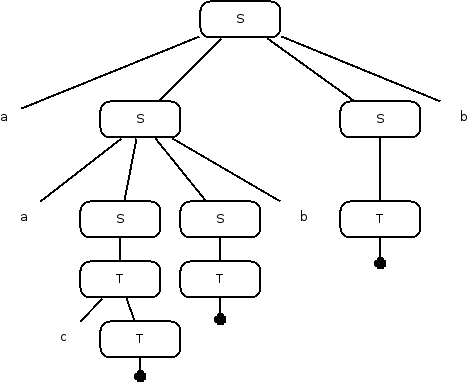
\includegraphics[width=0.7\linewidth]{../dia/derivation}
\end{center}

Une grammaire est \textbf{ambiguë} si il existe au moins un mot
qui peut être obtenu de différentes façons.

Exercice : montrez que la grammaire de l'exemple est ambiguë.

L'ambiguïté peut être une source de problèmes. Par exemple
pour l'analyse de expressions arithmétiques. La grammaire

$$\begin{array}{rcl}
E & \rightarrow &  E + E \\
 & \rightarrow &  E - E \\
 & \rightarrow &  E * E \\
 & \rightarrow &  E / E \\
 & \rightarrow &  ( E )  \\
 & \rightarrow & nombre
\end{array}
$$
reconnaît les expressions arithmétiques correctes, mais
fournit deux arbres de dérivation pour ``$1+2*3$'',
dont un qui ne correspond pas aux priorités habituelles.

\section{Langages algébriques}

Un langage est algébrique si il existe au moins une grammaire
context-free qui le reconnaît.

Exercices : donnez des grammaires, si possible non-ambiguës, pour les
les langages suivants :

\begin{enumerate}
\item $\{ a^n b^n, n \ge 0 \}$
\item mots qui ont autant de $a$ que de $b$
\item systèmes de parenthèses
\item expression arithmétique
\end{enumerate}

\paragraph{Remarques}
\begin{itemize}
\item Il existe des langages non-algébriques, comme 
$\{ a^n b^n c^n, n \ge 0 \}$
\item il existe des langages algébriques intrinséquement ambigus,
c'est-à-dire qui reconnus par des grammaires qui sont toutes ambigües.
Exemple  
$\{ a^n b^m c^p, n = m \mbox{ ou } m = p \}$
\end{itemize}

Une idée de la preuve pour le premier résultat: 
\begin{enumerate}
\item on peut transformer toute grammaire en une grammaire équivalente
dont l'axiome n'apparaît jamais en partie droite d'une règle (il suffit
de définir dont dérive l'ancien axiome)
et dont aucun non-terminal, sauf éventuellement l'axiome, ne produit le mot vide 
(on les remplace).
\item si on prend un mot $a^n b^n c^n$ assez long, son arbre de dérivation
aura une branche de taille supérieure au nombre de non-terminaux, et  
il y aura donc un non-terminal $N$ qui apparaît deux fois sur une branche.
De l'axiome $S$ dérive dont un mot $uNv$ ($u$ et $v$ suite de terminaux, 
qui ne sont pas tous les deux vides), 
d'où dérive encore $u u' N v' v$ qui produit $u u' w v' u$ qui 
appartient au langage.
\begin{center}
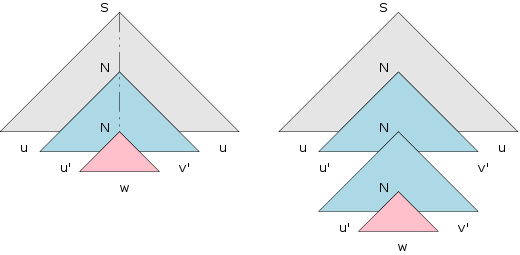
\includegraphics[width=.8\linewidth]{../dia/anbncn}
\end{center}
\item  on peut donc construire un autre mot dérivé en répétant la seconde
étape, c'est $u u' u'  w v' v' v$, dont il est facile de voir 
qu'il n'appartient pas au langage : si $u'$ (ou $v'$) contient deux types de lettres,
$u'u'$ contient une alternance de lettres. si $u'$ et $v'$ sont
des répétitions d'une même lettre, il y aura forcément un 
déséquilibre avec le nombre d'occurrences de la troisième lettre.

\end{enumerate}

\section{Automates à pile}

De la même manière que les langages rationnels sont reconnus par les
automates finis, les langages algébriques le sont par les automates 
à pile.

Qu'est-ce qu'un \textbf{automate à pile} ?

\begin{itemize}
\item il possède une \textbf{pile}, qui est une suite de symboles, don un mot sur un  vocabulaire
  de pile.  Par commodité, on considère que la pile vide est
  représentée par un symbole particulier, appelé ``fond de pile'' ($\bot$).
\item il possède des \textbf{états}, dont un état initial, et des états finaux.
\item il a des \textbf{transitions}, qui indiquent, en fonction 
d'une situation donnée, c'est à dire
\begin{itemize}
\item l'état courant,
\item une lettre du mot
\item le symbole qui est en sommet de pile
\end{itemize}
la nouvelle situation 
\begin{itemize}
\item le nouvel état
\item par quoi il faut remplacer le sommet de la pile
\end{itemize}
\end{itemize}

Il existe plusieurs types d'automates à pile, 
\begin{itemize}
\item mot reconnu si pile vide ou pas à la fin ?
\item
l'automate peut être
déterministe (pour un état, une lettre, un symbole, il a une seule
transition possible), ou non.  
\end{itemize}


\paragraph{Exemple d'automate}, pour reconnaître $a^n b^n$
\begin{itemize}
\item deux états : OK (initial) et ERREUR
\item symbole de pile : $c$. La taille de la pile sert de compteur.
\item transitions
\begin{center}
\begin{tabular}{|c|c|c||c|c|}
\hline
état &       &   sommet &    état &    à  \\ 
avant & lettre & de pile &   après &   empiler \\
\hline
NORMAL  & $a$  &  $\bot$ &    NORMAL  & $c \bot$ \\
NORMAL  & $a$  &  $c$   &   NORMAL  & $c c$ \\
\hline
NORMAL  & $b$  &  $\bot$ &  ERREUR &  $\bot$ \\
NORMAL  & $b$  &  $c$ &  ERREUR &  $\epsilon$ \\
\hline
ERREUR  & $a$ & $c$ & ERREUR & $\epsilon$ \\
ERREUR  & $b$ & $c$ & ERREUR & $\epsilon$ \\
ERREUR  & $a$ & $\bot$ & ERREUR & $\bot$ \\
ERREUR  & $b$ & $\bot$ & ERREUR & $\bot$ \\
\hline
\end{tabular}
\end{center}

Ici on dira qu'un mot est reconnu si, après avoir effectué toutes
les transitions, l'état est final et la pile est vide ($\bot$).
\end{itemize}


\paragraph{Exercice : } construire un automate pour les mots qui ont
autant de $a$ que de $b$. Idée : utiliser la pile comme compteur
du nombre de $a$ moins le nombre de $b$. Empiler des $p$ pour 
une valeur positive, et des $n$ quand c'est négatif.


\section{BNF}


La notation BNF (Backus Naur Form)  a été
introduite par John Backus et Peter Naur
 pour décrire le langage de programmation Algol 60.

Plus précisement, elle a été (en grande partie) inventée par
Backus pour décrire Algol 58 dans un rapport de recherche.
Et Peter Naur (qui travaillait sur le même langage) 
s'est alors aperçu qu'il voyait autrement
la syntaxe d'Algol 58.

Ils ont donc décidé, pour le travail
sur Algol, 
de distribuer des descriptions écrites de la 
syntaxe pour que tout le monde parle de la même chose
lors des réunions du groupe de travail. 

{\scriptsize
Source : \url{http://cui.unige.ch/db-research/Enseignement/analyseinfo/AboutBNF.html}}

\subsection{BNF de base}

La notation de base (historique) de la BNF est simple 
\begin{itemize}
 \item la chaîne ``\texttt{::=}'' signifie ``\emph{est défini par}'',
\item la barre \verb+|+ sépare des alternatives,
\item les chevrons ``\verb/<...>/'' entourent des noms de catégories,
\item les éléments terminaux sont représentés tels quels,
\end{itemize}
et se traduit directement en grammaire formelle.

\textbf{Exemple}
\begin{lstlisting}[frame=single]
<program> ::=  program
                   <déclarations>
               begin
                   <instructions>
               end ;

<instruction> ::=   <affectation>
                  | <instruction_tant_que>
                  | <instruction_si_alors_sinon>
                  | ...
\end{lstlisting}


Dans des textes plus modernes, on peut avoir d'autres conventions :
terminaux en gras ou en police ``machine à écrire'', non-terminaux
 en italique, etc.

\begin{center}
\emph{program} ::=  \textbf{program} \emph{declarations}
\textbf{begin} \emph{declarations} \textbf{end}
\end{center}

\subsection{Extensions}

Quelques extensions s'avèrent pratiques, elles sont notées
par des \emph{méta-caractères} :
\begin{itemize}
\item des \textbf{crochets} pour entourer les éléments optionnels
\begin{tabbing}
\hspace{3cm} \= \hspace{1cm}  \= \hspace{1cm} \\
\emph{instruction\_si\_alors\_sinon} ::= \\
  \> \textbf{if} \emph{condition} \\
  \> \> \textbf{then} \emph{instruction} \\
  \> \> [ \textbf{else} \emph{instruction} ]  \\
\end{tabbing}

\item des \textbf{accolades} pour les éléments répétés (zero ou plusieurs fois)
\begin{tabbing}
\hspace{3cm} \= \hspace{1cm}  \= \hspace{1cm} \\
\emph{liste\_d'expressions} ::= \\
  \> \textbf{( ) } \\
  \> | \textbf{(} \emph{expression} \{ \textbf{,} \emph{expression} \} \textbf{)}
\end{tabbing}
\item on peut aussi entourer les terminaux 
de guillemets.
\end{itemize}

\paragraph{Exercice :} comment définir les listes d'expressions en BNF de base, 
sans  ces méta-caractères ?

\paragraph*{Un exemple} plus complet, la syntaxe de la BNF ... en BNF

\begin{lstlisting}[frame=single]
syntax     ::=  { rule }
rule       ::=  identifier  "::="  expression
expression ::=  term { "|" term }
term       ::=  factor { factor }
factor     ::=  identifier |
                quoted_symbol |
                "("  expression  ")" |
                "["  expression  "]" |
                "{"  expression  "}"
identifier ::=  letter { letter | digit }
quoted_symbol ::= """ { any_character } """
\end{lstlisting}

\subsection{Exercices}
\paragraph{Le langage PL/0} de N. Wirth est décrit par une grammaire
de type E-BNF (extended BNF). Ecrivez quelques programmes dans ce langage.
{\small
\begin{lstlisting}[frame=single,numbers=left]
 program = block "." .
 
 block =
     ["const" ident "=" number {"," ident "=" number} ";"]
     ["var" ident {"," ident} ";"]
     {"procedure" ident ";" block ";"} statement .
 
 statement =
     ident ":=" expression
     | "call" ident
     | "begin" statement ";" {statement ";"} "end"
     | "if" condition "then" statement
     | "while" condition "do" statement .
 
 condition =
     "odd" expression
     | expression ("="|"#"|"<"|"<="|">"|">=") expression .
 
 expression = ["+"|"-"] term {("+"|"-") term} .
 
 term = factor {("*"|"/") factor} .

 factor =
     ident
     | number
     | "(" expression ")" .

\end{lstlisting}

\paragraph{Exercice.} Voici des exemples de déclarations de type en 
langage Pascal. Fournissez une grammaire qui couvre au moins
les exemples :

\begin{verbatim}
type chaine = array [1 .. 30] of char;
type date = record 
               jour : 1..31;
               mois : 1..12;
               annee : integer
            end;
type personne = record
                  nom, prenom : chaine;
                  naissance   : date
                end;
\end{verbatim}
Notez qu'en Pascal le point-virgule est un séparateur, alors qu'en C c'est un 
terminateur. Il est donc facultatif après le dernier élément d'un \emph{record}.

                   
\paragraph{Exercice. } Voici un programme écrit dans un langage jouet
\begin{verbatim}
function fac(n)
  local r = 1, i
  for i = 1 to n do
    let r = r * i
  endfor
  return r
endfunction

let encore = 1
while encore == 1 do
  print "valeur de n ? "
  read n
  if n < 0 
  then 
     print "n est négatif"
     let encore = 0
  else 
     let r = fac(n)
     print "factorielle ", n, " = ", r
  endif
endwhile  
\end{verbatim}

Fournir une description du langage en BNF étendue.


\section{Diagrammes syntaxiques}


Les diagrammes syntaxiques expriment essentiellement la même chose que la BNF
mais sous une forme plus facile à appréhender

Exemple : les expressions arithmétiques.

{\scriptsize

\url{http://commons.wikimedia.org/wiki/File:Diagrammes_Syntaxiques.png}
}

\begin{center}
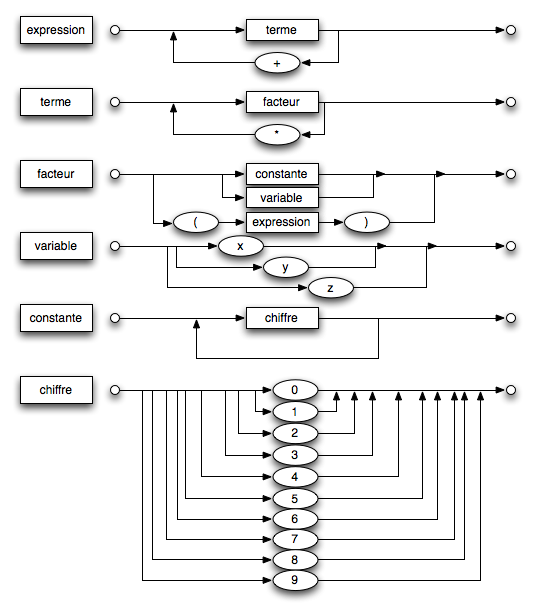
\includegraphics[width=\linewidth]{../images/Diagrammes_Syntaxiques}
\end{center}

Les diagrammes syntaxiques peuvent être vus comme des programmes
(visuels) qui décrivent l'analyse d'une chaine de caractères, en
termes d'appels de sous-programmes : pour reconnaître une expression,
il faut d'abord reconnaitre un terme. Pour reconnaitre un terme
il faut d'abord reconnaitre un facteur, etc.

C'est la base de la technique d'analyse récursive descendante,
technique élégante qui a été appliquée dans nombre de compilateurs
``écrits à la main''\footnote{En effet, une autre option est d'utiliser un programme qui fabriquera un
automate à pile à partir d'une grammaire du langage à reconnaitre.}

\subsection{Déterministe ou pas ?}

A certains endroits du diagramme il y a des fourches, ce qui laisse craindre
un non-déterminisme. Par exemple, dans
\emph{constante}, si on rencontre un second \emph{chiffre}, doit-on 
boucler, ou sortir ?

De préférence, on voudra un analyseur déterministe, il faut donc
étudier la grammaire sous-jacente pour montrer qu'on n'a en fait
jamais le choix.

\paragraph{Méthode. } on regarde en particulier 
\begin{itemize}
\item l'ensemble $First(N)$ 
des terminaux qui peuvent apparaître en première position d'un
non-terminal $N$.
\item l'ensemble $Follow(N)$ 
des terminaux qui peuvent apparaître après un
non-terminal $N$.
\end{itemize}

\paragraph{Pour \emph{First},} on a évidemment 
\begin{itemize}
\item $First(Chiffre) = \{ 0 .. 9 \} $ 
\item et 
$First(Variable) = \{ x, y, z \} $.
\item et donc $First(Constante) = First(Chiffre) = \{ 0 .. 9 \} $
\end{itemize}
Par conséquent, les trois branches de la fourche d'entrée de
\emph{facteur} correspondent à des cas disjoints (le troisième est une
parenthèse ouvrante), le choix peut même se faire en regardant
seulement un seul caractère de la chaîne d'entrée.

\paragraph{Pour \emph{Follow.}}
Les flèches de boucle posent la question de savoir si un ``+''
peut suivre une \emph{expression}, une étoile un terme, un chiffre une
constante. Donc de savoir dans quels contextes on peut rencontrer ces
non-terminaux, \emph{dans une chaîne valide}.

On suppose donc que le but est d'analyser une expression isolée, donc
qu'on a une règle liant l'axiome$S$, les expressions et $\$$ une
marque de fin.
$$ S \rightarrow  \mbox{expression} \ \$ $$
De cette règle en déduit immédiatement que
$$\$ \in Follow(expression) $$

Du troisième diagramme, on tire aussi qu'une parenthèse 
fermante (notons-l $f$)
peut suivre une expression : $f \in Follow(expression) $.

Un certain nombre d'inclusions se déduisent également :
si un symbole peut suivre une expression, alors
il peut aussi suivre un terme (diag. 1). Un plus peut aussi suivre un terme.


\subsection{Un systeme d'inequations}

\paragraph{Le tableau ci-dessous} résume nos trouvailles

\begin{center}
\begin{tabular}{|l|rcl|}
\hline
origine &  & \\
\hline
axiome & $\$ $& $\in $&$ Follow(expression)$ \\
diag. 1  & $Follow(expression)$ & $\subseteq $&$  Follow(terme)$ \\
diag. 1  & $"+"$ & $\in  $&$ Follow(terme)$ \\
\hline
diag. 2  & $Follow(terme)$ & $\subseteq $&$  Follow(facteur)$ \\
diag. 2  & $"*"$ & $\in $&$  Follow(facteur)$ \\
\hline
diag. 3  & $Follow(facteur) $&$ \subseteq $&$  Follow(constante) $\\
diag. 3  & $Follow(facteur) $&$ \in $&$  Follow(variable) $\\
diag. 3  & $f$ & $\in $&$  Follow(expression)$ \\
\hline
diag. 4  & $First(chiffre) $ & $ \subseteq $&$  Follow(chiffre) $\\
diag. 4  & $First(constante) $&$ \subseteq $&$  Follow(chiffre) $\\
\hline
\end{tabular}
\end{center}

C'est un système d'inéquations sur des ensembles ; nous en cherchons les 
plus petites solutions.

Pas de panique, la résolution n'est pas compliquée, elle se fait par
un algorithmes itératif :
\begin{itemize}
\item on part d'ensembles vides $E, T, F, Co, V, Ch$ qui représentent
les différents ``follow''.
\item on exécute une boucle qui interprète chaque inéquation comme
une affectation 
\begin{itemize}
\item la première ajoute $\$$ à $E$
\item la seconde ajoute le contenu de $E$ à $T$,
\item etc. 
\end{itemize}
\item il n'y a qu'un nombre fini de symboles, et on ne fait qu'ajouter des éléments, au bout d'un certain
nombre de tours la situation va se stabiliser : on s'arrête.
\end{itemize}


\subsection{Use the computer, Luke}

L'ordinateur qui est votre ami va calculer la solution
en moins de deux, si on écrit un programme Python comme celui-ci
\begin{lstlisting}[language=python, frame=single, numbers=right]
from copy import deepcopy

F = { "e" : { "dollar", "fermante"}, 
      "t" : { "+"}, 
      "f" : { "*" }, 
      "co" : set(), 
      "v" : set(), 
      "ch" : {"chiffre"} }

def m(src, dst):
  F[dst].update(F[src])

n = 0
while True :
  n = n + 1
  old = deepcopy(F)
  m("e", "t")
  m("t", "f")
  m("f", "co")
  m("f", "v")
  m("co", "ch")
  if old == F : break

print ("arret apres %d iterations" % n)
for k in F:
  print (k + " => " + str(F[k]))
\end{lstlisting}

On obtient le résultat
\begin{lstlisting}
arret apres 2 iterations
ch => set(['chiffre', '*', 'dollar', 'fermante', '+'])
co => set(['+', '*', 'dollar', 'fermante'])
f => set(['fermante', '+', '*', 'dollar'])
t => set(['fermante', '+', 'dollar'])
v => set(['+', '*', 'dollar', 'fermante'])
e => set(['dollar', 'fermante'])
\end{lstlisting}

Donc, résumons, les diagrammes syntaxiques sont déterministes parce que
\begin{itemize}
\item après une expression il ne peut pas y avoir un ``+'' (diag. 1)
\item un facteur ne peut pas être suivi par ``*'' (diag. 2)
\item une constante ne peut pas être suivie par un chiffre (diag. 3)
\end{itemize}

\subsection{Compléments}

\begin{itemize}
\item Ici nous avons montré qu'on peut choisir son chemin 
dans le diagramme de l'exemple, en regardant seulement le prochain
caractère de la chaine à analyser.

Certains langages nécessitent de regarder plusieurs caractères. 

\item En C, C++,
c'est même plus compliqué : le nombre d'éléments à lire pour différencier,
par exemple, une affectation d'un appel de fonction n'est pas borné. 
Voyons par exemple 
\begin{verbatim}
 f(....);
 g(....)->a = b; // g fonction qui retourne un pointeur
\end{verbatim}
et l'analyse syntaxique doit donc se baser également sur les types
déclarés.

\item Le calcul de $First$ et $Follow$  est un petit peu plus compliqué
quand les non-terminaux peuvent produire un mot vide. Si on a une règle
$$A \rightarrow B C $$, $First(A)$ contient $First(B)$, mais aussi
$First(C)$ si $B$ peut produire le mot vide. Et aussi $Follow(A)$ si
$B$ et $C$ produisent le vide.

$First(A)$ doit alors être interprété comme ``le premier symbole que
je peux rencontrer si je vais vers un bloc $A$ dans le diagramme''.
\end{itemize}

Tout ceci est fort intéressant et mérite d'être étudié de plus près,
vous en saurez plus si vous continuez en Mastère ou Ecole d'ingénieur
d'informatique.

\section{Descente récursive, un exemple}

Le programme ci-dessous analyse une expression arithmétique, et en fournit
une paraphrase.

Voici le résultat des tests

\lstinputlisting[frame=single,breaklines=true]{../src/lecture-expr.run}

et le source dans les pages qui suivent.

\begin{landscape}

\lstinputlisting[language=c++,frame=single,numbers=left,breaklines=true]{../src/lecture-expr.cxx}

\end{landscape}




\end{document}



